\documentclass[11pt]{article}
\usepackage[top=1.00in, bottom=1.0in, left=1.1in, right=1.1in]{geometry}
\renewcommand{\baselinestretch}{1.1}
\usepackage{graphicx}
\usepackage{natbib}
\usepackage{gensymb}
\usepackage{amsmath}
\usepackage[utf8]{inputenc}
\usepackage{lineno}
\usepackage{xr-hyper}
% \externaldocument{limitingcues_supp}

\def\labelitemi{--}
\renewcommand{\baselinestretch}{1.2}
\parindent=0pt
\parskip=5pt




\title{Unravelling the phenology-phylogeny tangle.}
% alternative titles:
%% An expanded bayesian phylogenetic mixed model to unravel the phenology-phylogeny tangle. %% this sounds too methodsy
\usepackage{Sweave}
\begin{document}

\maketitle

\noindent Authors:\\
The Wolkovich Lab in 2019 \& collaborators $^{1,2,3,4}$ % Will Pearse, Jonathan Davies also
\vspace{2ex}\\
\emph{Author affiliations:}\\
$^{1}$Forest \& Conservation Sciences, Faculty of Forestry, University of British Columbia, 2424 Main Mall, Vancouver, BC V6T 1Z4;\\
$^{2}$Arnold Arboretum of Harvard University, 1300 Centre Street, Boston, Massachusetts, USA;\\
$^{3}$Organismic \& Evolutionary Biology, Harvard University, 26 Oxford Street, Cambridge, Massachusetts, USA;\\
$^{4}$Edificio Ciencias, Campus Universitario 28805 Alcal<U+00E1> de Henares, Madrid, Spain\\
 

\vspace{2ex}
$^*$Corresponding author: ignacio.moralesc@uah.es\\
\renewcommand{\thetable}{\arabic{table}}
\renewcommand{\thefigure}{\arabic{figure}}
\renewcommand{\labelitemi}{$-$}
\setkeys{Gin}{width=0.8\textwidth}

\clearpage

%%%%%%%%%%%%%%%%%%%%%%%%%%%%%%%
% Results & Discussion
%%%%%%%%%%%%%%%%%%%%%%%%%%%%%%%

List of 7
 $ y    : num [1:4418] 56.4 52.2 59.6 49.2 61.5 ...
 $ chill: num [1:4418] 0.05623 0.00346 0.05623 0.00346 0.05623 ...
 $ force: num [1:4418] -1.8 -1.8 -1.8 -1.8 -1.8 ...
 $ photo: num [1:4418] -0.721 -0.434 -0.721 -0.434 -0.721 ...
 $ sp   : num [1:4418] 1 1 1 1 1 1 1 1 1 1 ...
 $ N    : int 4418
 $ n_sp : int 234
[1] "Unique forcing types are ..."
[1] "ramped" "exp"    "amb"   
[1] "Unique photo types are ..."
[1] "ramped" "exp"    "amb"    "none"  
[1] "Unique chilling types are ..."
[1] "fldest"  "bothest" "bothrep" "exp"    
[1] "Range of chilling is ..."
[1] -3.248548  4.525265

Number of species in tree before: 0
Number of species in tree now:    24 
***************************************************************
*                          Note:                              *
*    force.ultrametric does not include a formal method to    *
*    ultrametricize a tree & should only be used to coerce    *
*   a phylogeny that fails is.ultramtric due to rounding --   *
*    not as a substitute for formal rate-smoothing methods.   *
***************************************************************
[1] "n_eff / iter looks reasonable for all parameters"
[1] "Rhat looks reasonable for all parameters"
[1] "0 of 8000 iterations ended with a divergence (0%)"
[1] "0 of 8000 iterations saturated the maximum tree depth of 10 (0%)"
[1] "E-BFMI indicated no pathological behavior"
\section*{Results \& Discussion}
% Are we in past or present tense here? (asks Lizzie)

Most species are sensitive to all three primary cues---forcing, chilling, and photoperiod (Figs. \ref{fig:muplot_all}, Supporting Table \ref{tab:})\citep[see also][]{Laube:2014a,ettinger2020}---with sensitivity to chilling approximately five-fold greater than sensitivity to photoperiod, on average (phenological advances of 7.2 days per standardized unit vs 1.4 days, for chilling and photoperiod, respectively; see Table \ref{tab:modelanglamb}). However, these average sensitivities estimated across species, fail to capture the large differences in species' responses to chilling and forcing (Figs. \ref{fig:muplot_all}, Supporting Table \ref{tab:}). 

By allowing species responses to vary, based on a model including their shared evolutionary history, we found species differences dwarfed differences between cues, especially temperature cues (Fig. \ref{fig:muplot_all}). The largest in magnitude cue---chilling---varied 25-fold between species, while variation to forcing varied 6-fold. These results suggest the strong focus on comparing cues may miss the largest variation. Robust phenological forecasts must then account for both the complexity of multiple cues and species-level variation in responses to them.

\emph{Differences across clades \& cues}

The large differences across species generally occurred coherently within clades, producing striking differences between clades. Oaks and beeches (Fagaceae), elms (Ulmaceae) and buckthorns (Rhamnaceae) are highly sensitive to chilling while rhododendrons (Ericaceae), butterfly bushes (Scrophulariaceae) or spindles (Celastraceae) show little to no response to chilling (Fig. \ref{fig:muplot_all} a). %IMC: not sure if we need some natural history here or some mention to research for some of these clades. Lizzie, if you want to mention-cite something here, please jump in. % EMW (21Nov2022 and 1 Dec2022) I can work with JD to add more here later.
% JD I think some biogeography may be useful here, for example, I think rhododendrons & buddleia are native to the Himalaya, but both are also now widespread and invasive ... need to do a little more digging on the exact species.   
Similar clade-level variation was observed for forcing, where some of these clades---e.g., Ericaceae, Rhamnaceae, Ulmaceae, or Fagaceae---were particularly sensitive (advancing their budburst more than 10 days per standardized unit of forcing) and others such as the Sapindaceae, Cornaceae or Juglandaceae families show little response (Fig. \ref{fig:muplot_all} b). %JD - perhaps could link back to invasiveness? Species more sensitive to forcing more invasive?

Some species responded strongly to both temperature cues (chilling and forcing), which could suggest the existence of syndromes where the genetic basis for responses to one cue (e.g., forcing) has been been selected for alongside responses to another cue (e.g. chilling). We might expect, for example, early-season species to be sensitive to multiple cues as mistiming phenology could result in exposure to harsh conditions, leading to tissue loss or death \citep{frostbook}, and sensitivity to multiple cues likely provides greater insurance against mistiming \citep{memegan2021}. Alternatively or additionally, linkage or pleiotropism among loci associated with sensitivity to different cues \citep{nakagawa2005} could induce correlated cues. However, the correlation in species sensitivities across cues was weak (\emph{r} = 0.31; between forcing an chilling) and some genera, such as \emph{Tilia} and Ericaceae[genus?], displayed strong responses to forcing but weak responses to chilling, while others, such as XXXXExamplesXXXX, show strong responses to chilling but weak responses to forcing (Fig. \ref{fig:muplot_all}). Species sensitivity to one cue, thus, does not constrain sensitivity to another cue, and selection might operate independently on responses to different cues \citep{bonamour2019}.

In contrast to both chilling and forcing, species-level responses to photoperiod were almost uniform---present across nearly all species. This provides novel insight on a large debate over the prevalence of photoperiod cues in temperate trees, where previous experiments  \citep{Basler:2012,zohner2016} and modeling exercises \citep[e.g.,][]{Hunter:1992jw,schaber20203} suggested important variability across species that may constrain the responses of certain species to warming \citep{way2015}. Our results suggest variability is limited to a handful of species in Fagaceae, which have been heavily studied, especially \emph{Fagus sylvatica} \citep[e.g.,][]{Basler:2012,zohner2016,kramer2017}. These same few species are also where most evidence of local adaptation in photoperiod cues for spring phenology comes from \citep[e.g.,][]{kramer2017}, in contrast with common garden studies of other species, which found little evidence of local adaptation in spring (but not fall) phenology \citep{aitken2016}. The uniformity of response to photoperiod that we found supports this latter view of generally low local adaptation in photoperiod cues for spring phenology: given that studies spanned a range of latitudes (with many species studied in only a narrow latitudinal range), if local adaptation was high in photoperiod cues we would expect more variability across species. 

Our results suggest that while chilling and forcing are the dominant cues in terms of the magnitude of their effect sizes, most species are also sensitive to photoperiod, highlighting the potential importance of this cue to both climate change responses in the future, and through evolutionary history. In plants, photoperiod regulates a number of fundamental processes including growth, flowering, stress tolerance, and circadian rhythm \citep{serrano2017,Singh:2017}, with photoperiodic sensing and adaptation to shifting daylength likely occurred early in the evolution of plants, with origins in the green algae \citep{serrano2017}. It is possible, therefore, that phenological responses to photoperiod reflect ancestral sensitivities with origins in deep time. Large plasticity in responses to additional environmental cues (e.g., temperature) for a given photoperiod cue \citep[e.g.,][]{kramer1995} may allow species to track interannual variation in climate with little directional selection on photoperiod sensitivities. Alternatively, photoperiod might thus provide a reliable calibration of the underlying biological clock \citep{jackson2009plant} upon which seasonal variation in climate modifies the tempo. 
%JD - I still need to get to grips with what is going on with photoperiod, low lambda is consistent with rapid evolution within species, but low sigma suggests low rates of evolution. Perhaps photoperiod is dominated by local adaptation, but little directional selection, so local adaptation just gets washed out overtime?

\emph{Phylogenetic structure of phenological cues}

Variation---or lack thereof---in cues across species and clades, alongside related estimates from our modeling approach, provides possible insights into the evolution of cues across the phylogeny. While responses to each cue were phylogenetically structured, the strength of phylogenetic conservatism in response differs between cues (Fig. \ref{fig:phylosig_all}). Responses to temperature (forcing and chilling) were moderately structured ($\lambda = 0.65$ and $\lambda = 0.54$, for forcing and chilling, respectively), with closely related species exhibiting more similar sensitivities than distantly related species. Phylogenetic structure in species responses to photoperiod was comparatively weaker ($\lambda= 0.39$) (see Fig. \ref{Fig:muplot_all}, Table \ref{tab:modelanglamb}), emphasizing again that photoperiod diverges from other climate cues. In addition to being weaker and more uniform across species, sensitivity to photoperiod appears to also be less evolutionarily constrained than sensitivities to temperature cues. % While our approach is unique in focusing on species cues, our results support previous work showing phylogenetic signal in plant phenological timing observed from floras or long-term data \cite{kochmer1986constraints,davies2013phylogenetic}. 

What might drive phylogenetic structure in species temperature responses? Differences between species in their responses represent shifts in the slope of the relationship between the observed phenology and the cue. Thus, the observed phylogenetic structure in temperature responses (forcing and chilling) would be consistent with an interaction with a non-measured trait that moderates responses, and which also covaries with phylogeny \citep{davies2019phylogenetically}. This fits fundamentally with the idea that early-season phenology plays a critical role in shaping species temporal niches \citep{gotelli1996} and thus should covary with a suite of life-history traits, including whether species are early-active with rapid return on investment trait, or start later in the season and have traits associated with higher competitive abilities \citep[e.g.,][]{Grime:1977sw,wolkovich2014aob}. Geography may drive structured phylogenetic variation, especially in regions where clades have radiated such that close relatives have experienced the same suite of environmental cues and thus been subject to similar selection regimes. Conversely, if species are not generally geographically constrained, as may be more likely the case, especially across deep time \citep{fitzturelli2006}, then we might expect phylogenetic structure in phenology to also weaken, especially when aggregating across locations with different cues \citep{davies2013phylogenetic}.

% EMW (21Nov2022): Do we want to mention any molecular work on photoperiod (or other cues)?
Weak phylogenetic signal in photoperiod sensitivity (Fig. \ref{fig:phylosig_all}) might seem at odds with observations that distantly related species respond more similarly (and less variably) to photoperiod than they do to forcing or chilling. However, somewhat counterintuitively, both uniform and random responses can manifest as low phylogenetic signal when estimated by Brownian motion expectations (see Wiens et al.). Rapid local adaptation within species might thus erase the phylogenetic structure in photoperiod responses, but seems at odds with the uniformity we find in species' responses. Alternatively, if responses to photoperiod evolved early in plants, as we suggest above, and subsequent selection on photoperiod sensitivity was constrained by stabilizing selection operating on other life-history attributes sensitive to photoperiod \citep[e.g.,][]{Rinne:1994,Wilczek2014,azeez2015}, we would predict both low interspecific variation and weak phylogenetic signal in responses, matching observations. This latter interpretation is also consistent with our estimates of lower $\sigma$ for photoperiod responses (CITE FIGURE). Here, as in more traditional phylogenetic comparative methods, $\sigma$ represents the rate of evolution, and thus our results suggest photoperiod responses are also evolving slower than temperature responses. However, we also show (see Appendix XXX) that an early burst model of evolution, in which trait variation accumulates rapidly early in the history of a clade and then slows through time, consistent with our interpretation of photoperiod evolution.
%JD - Call out to Will for assistance ...

Phylogenetic conservatism (high $\lambda$) and slow evolutionary rates (low $\sigma$) in traits has sometimes been interpreted as indicative of evolutionary constraints to adaptive change (cite Wiens et al. and others cites XXX). If this were the case, we might then suggest that species with strong forcing response might be more vulnerable to future warming because phylogenetic conservatism ($\lambda$) in responses to forcing is higher compared to other cues, and it evolutionary rate ($\sigma$) is lower. This is misleading, however, as estimates of $\lambda$ are independent from the rate of evolution, and macroevolutionary rates estimated on phylogenetic trees that integrate across millions of years of evolutionary history, and thus do not necessarily inform us of maximum possible rates of evolution over much shorter timescales. Indeed, there is accumulating evidence for rapid evolution to shifting climates \citep{bradshaw2006,franks2014}. Our estimates of phylogenetic structure are thus more useful in improving our understanding of the evolutionary history of species phenological cues, and show the importance of robustly estimating species differences in ecological forecasts. 

% I'm commenting out this bit but leave it here in case we want to mention some of it in methods or an appendix
%From a statistical perspective, accounting for the effects of phylogenetic structuring on the effects of jointly modelled cues had an effect on model coefficients (Fig. \ref{fig:correls_angio}). Not accounting for phylogeny (or assuming $\lambda$ = 0) biased model coefficients, particularly so for forcing and somewhat less for chilling (Fig. \ref{fig:correls_angio}). Specifically, species sensitivities to forcing and chilling were underestimated on average (model slopes shifted by 7.2\% and 3.7\%, respectively). Sensitivities to photoperiod, which showed weak phylogenetic signal were not biased in non-phylogenetic models (Fig. \ref{fig:correls_angio}), likely associated to their low estimated $\lambda$ values. Model intercepts were not affected either (Fig. \ref{fig:correls_angio}).\\ 

\emph{Forecasting species-level responses}

Our results highlight that species-level variability can be extremely high---when properly estimated. Our approach, which partially pooled species responses based on their shared evolutionary history, did not have major effects on the overall average across species (model slopes for forcing and chilling shifted by 7.2\% and 3.7\%, respectively; Fig. \ref{fig:correls_angio}), but estimated substantially higher variation across species compared with widely used hierarchical models. This was especially noticeable in temperature responses (for chilling variance across species was $\beta_{phylo}$ = 23.45 compared to $\beta_{non-phylo}$ = 17.47, for forcing it was $\beta_{phylo}$ = 8.74 compared to $\beta_{non-phylo}$ = 5.01) while photoperiod, which had low phylogenetic structure was more similar across approaches (variance of $\beta_{phylo}$ = 0.82 compared to $\beta_{non-phylo}$ = 0.93). Counterintuitively, induced reductions in cross-species variance, far from increasing estimation accuracy could lead to increased type-II error by failing to detect actual relationships among cue and responses that would only emerge when phylogeny is correctly accounted for (see Supporting Information XX). % EMWDec1 -- I am not sure what we mean in this last sentence, but it sounds important ... but since I am not sure what we mean I apologize if I put it in the wrong place 

% EMWDec2 -- not the most striking improvements! Might be better to remove these and just point to a figure ... but at least this gives a reminder of how to use \Sxpr (Sweave)
The increase in variability across species in our model with phylogenetic structure decreased the uncertainty in estimates for each  individual species temperature responses (by 6\% for chilling, 6\% for forcing and 2\% for photoperiod). Thus, traditional approaches that partially pool across species (most hierarchical models in ecology) may also lead to less precise predictions and forecasts of phenology for individual species, although overall model accuracy might still appear reasonable (see Appendix XX in Supporting Information).

% EMWDec1 -- need to check below about oaks and make sure we see this difference in lamba0 models... (and we could perhaps contrast this oak bit a little more)
Our results could help inform which clades will be more sensitive to different axes of climate change---e.g., changes temperatures over winter (associated with chilling) versus spring (associated with forcing). For example, using a hierarchical model would not have identified oaks (genus \emph{Quercus}) as being among the most sensitive taxa to forcing and chilling (see e.g., \citep{ettinger2020}), but we show that species within this genus advance phenology by 2 days per standard unit of forcing and 4 days per standard unit of chilling. These results highlight the need to move beyond current very general classifications currently used in models \citep[e.g., functional groups ... Cat/Dan, can you offer better ref?][]{Moorcroft:2003dz} or groupings at coarse taxonomic levels \citep[e.g.,][]{ettinger2020} to make improved ecological forecasts for individual species. 

The contrasts between temperature sensitivities and photoperiod sensitivities---in both their variability across species and phylogenetic structure---also allow for improved multi-species forecasts. For temperature responses, the large variability among species makes predicting species individual responses challenging, but the phylogenetic structure in responses lets us borrow  information from close relatives to improve our predictions. While this must be done with care \citep{molina2018assessing}, especially given our very limited sampling of species, our results could provide reasonable predictions for many temperate woody plant species from clades for which we have multiple species and experimental observations at varying treatment levels. For photoperiod, the weak phylogenetic structure in responses indicates that phylogeny retains little information, but because species responses are generally more uniform, we can be more confident in assuming the mean species response across species, comforted in the knowledge that small errors will likely not have large impact given the relatively weak overall contribution of this cue, except for \emph{Fagus sylvatica}. As \emph{Fagus sylvatica} is nearly five times more sensitive to photoperiod than most other measured tree species, our results caution against using it to draw inferences of photoperiod responses more widely. 
% The genus \emph{Fagus} is recognized as being particularly sensitive to photoperiod \citep{fu2019}. Specifically, \emph{Fagus sylvatica} is nearly five times more sensitive to photoperiod than most other measured tree species. The question arises as to whether species with outlying responses should be chosen as the model from which to extrapolate knowledge as done with \emph{Fagus sylvatica} in the phenology literature (REFs for PEP75?!). %HELP with references on Fagus would be appreciated. % EMW (21Nov2022) I'll add more here later

While we focused on spring phenology here, our modeling approach suggests a path towards more robust forecasting via useful species-level estimates of climate change responses. Our results show how including the phylogenetic relationship of species can overcome major limitations of most current hierarchical models (producing biased model estimates, underestimating the full variability across species, and increasing uncertainty around individual species' estimates) while at once providing insight into the evolutionary history of biological responses. [And, bam, something a little more here ... ]


\bibliography{phylorefs}
\bibliographystyle{amnat}


%%%%%%%%%%%%%%%%%%%%%%%%%%%%%%%
% Tables and Figures
%%%%%%%%%%%%%%%%%%%%%%%%%%%%%%%
\clearpage
\section*{Tables and Figures} 


%IMC 22mar - we should decide among one of the next two figures, instead of having separate figures per cues?
% EMW (28Mar2022): I vote for the first one, but both are great!
\begin{figure} [H]
  \begin{center}
  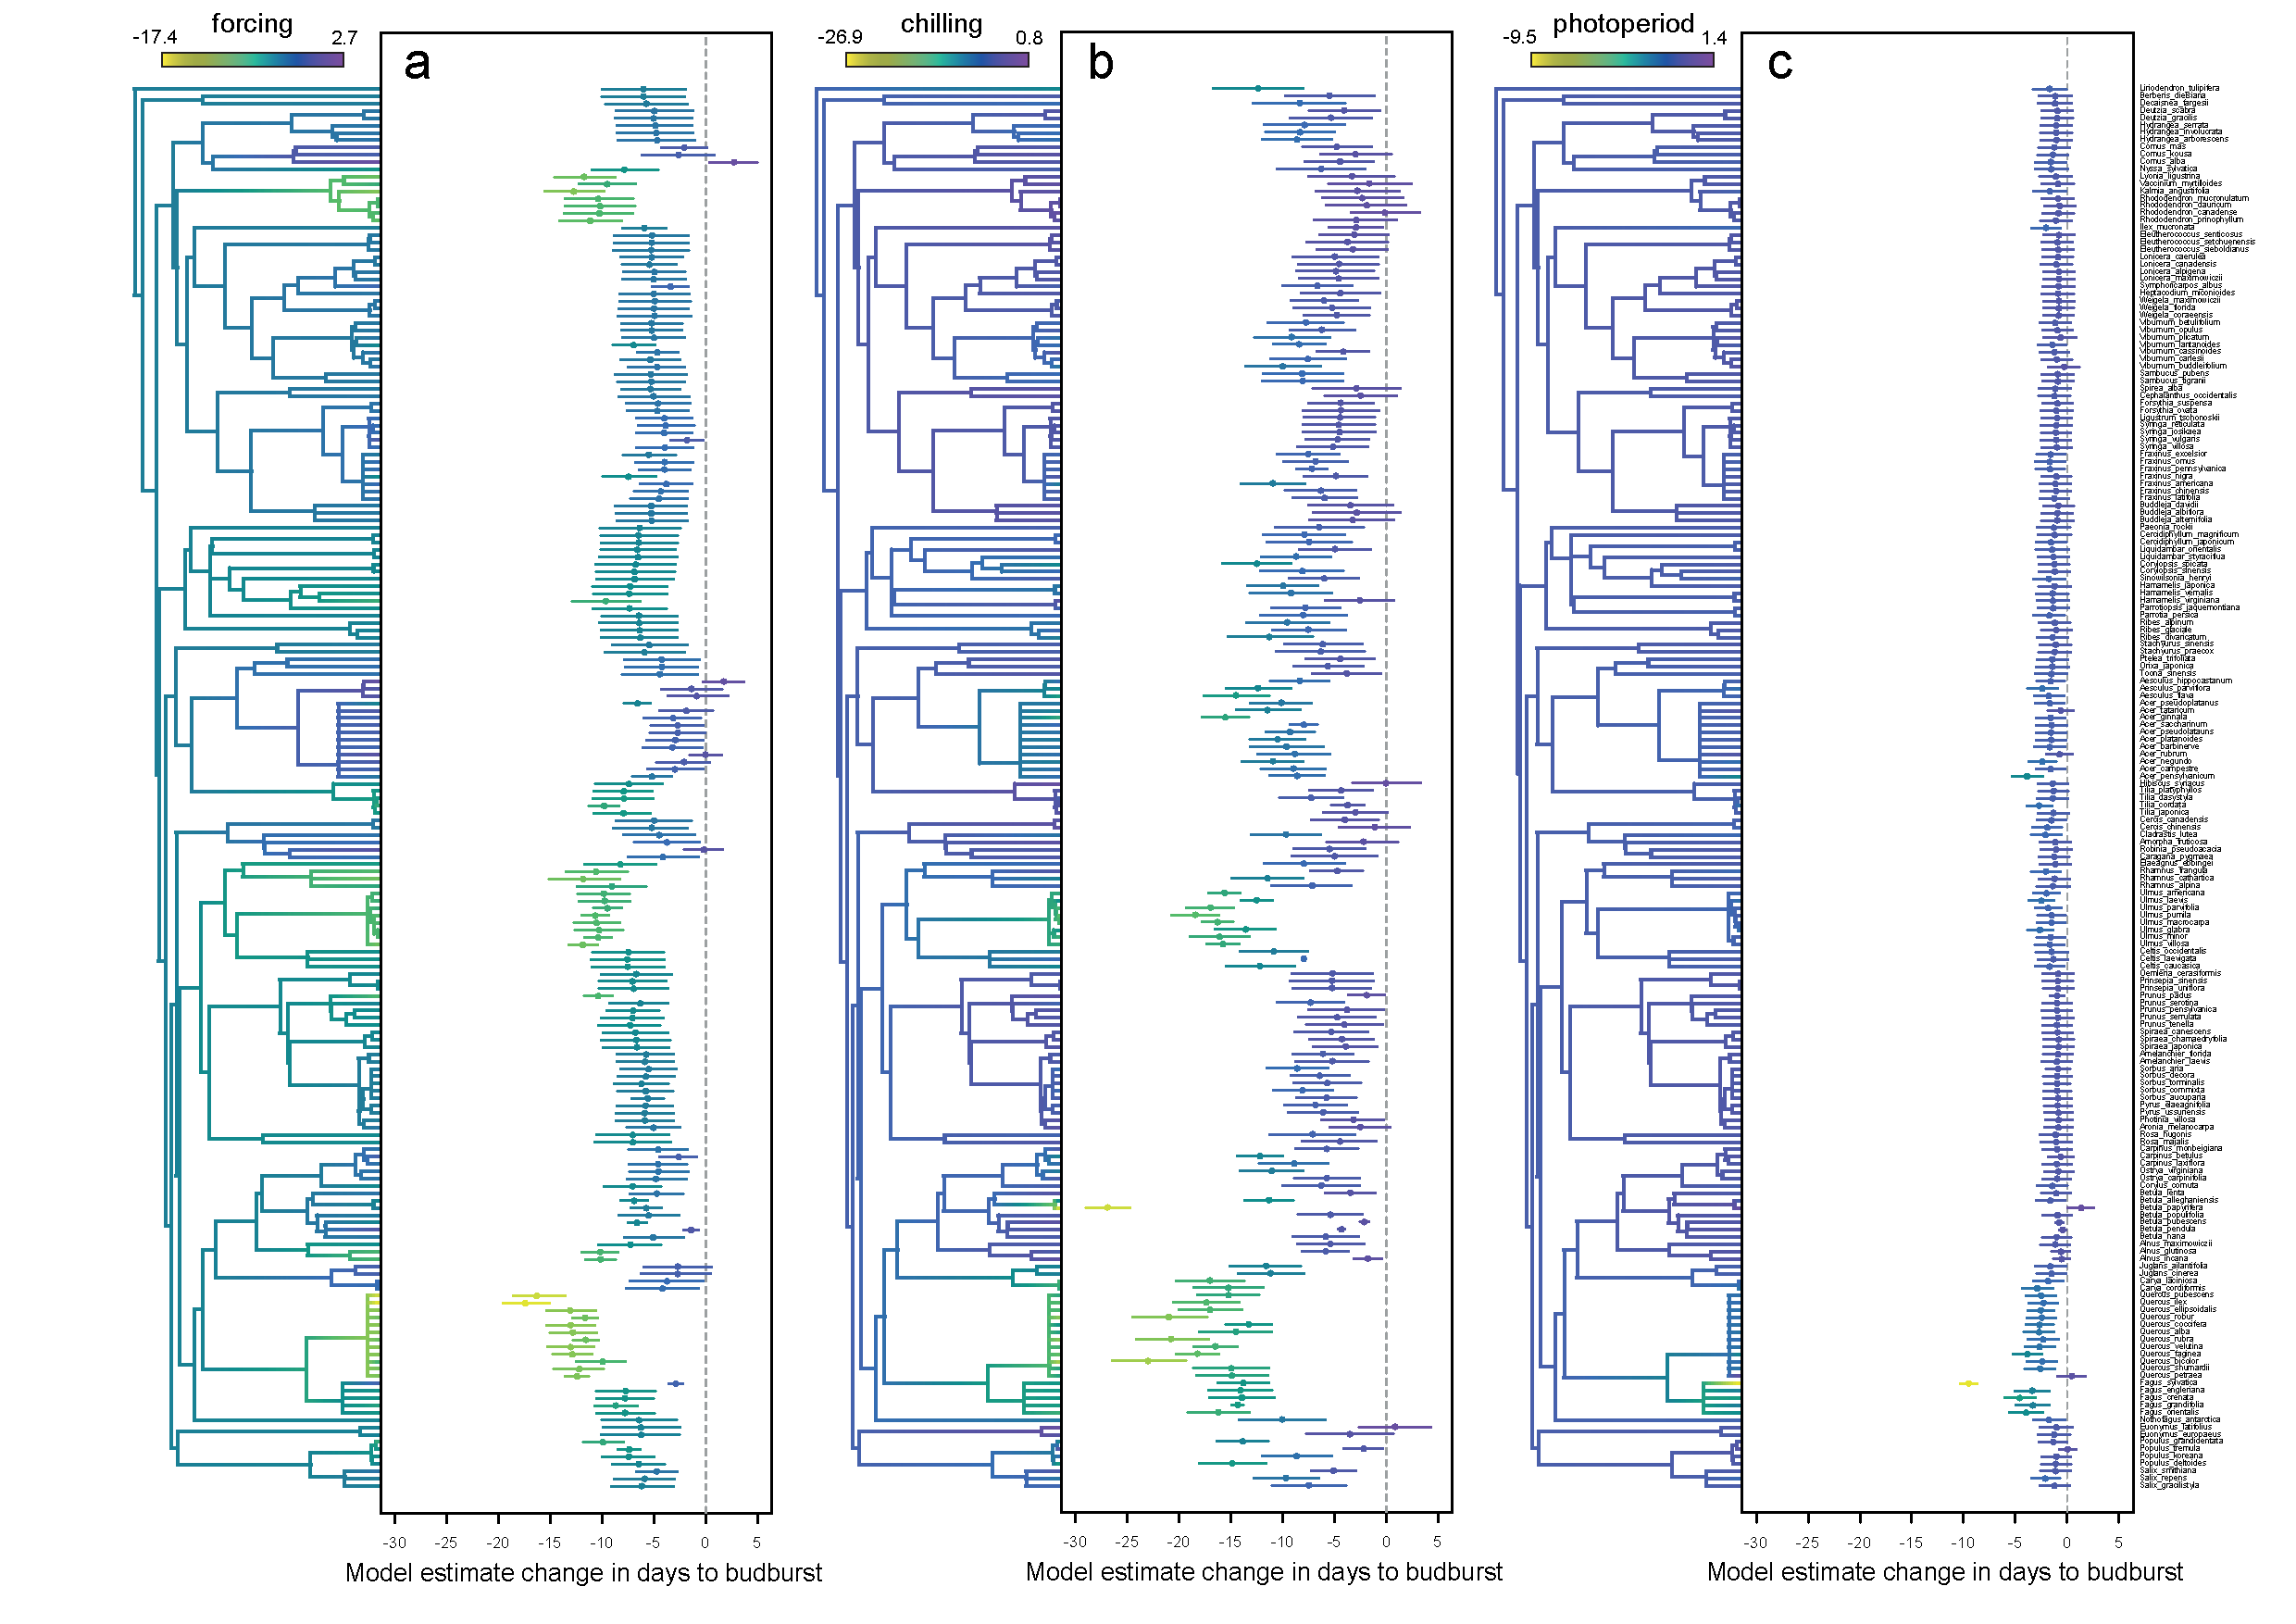
\includegraphics[width=16cm]{../../analyses/phylogeny/figures/muplot_phylo_allcue_angio.pdf}
  \caption{Phenological sensitivity to thee environmental cues, forcing (a), chilling (b) and photoperiod (c) measured in change in days to budburst per standardized unit (z-transformation) of the cues across 192 angiosperm species. The same phylogenetic tree is shown in each panel, colored acording to an estimation of ancestral character states, being the states at the tips the model slopes of our hierarchical phylogenetic model. Note that the color scale varies in each panel. Total tree depth is 81. My.}
  \label{fig:muplot_all}
  \end{center}
\end{figure}

\begin{figure} [H]
  \begin{center}
  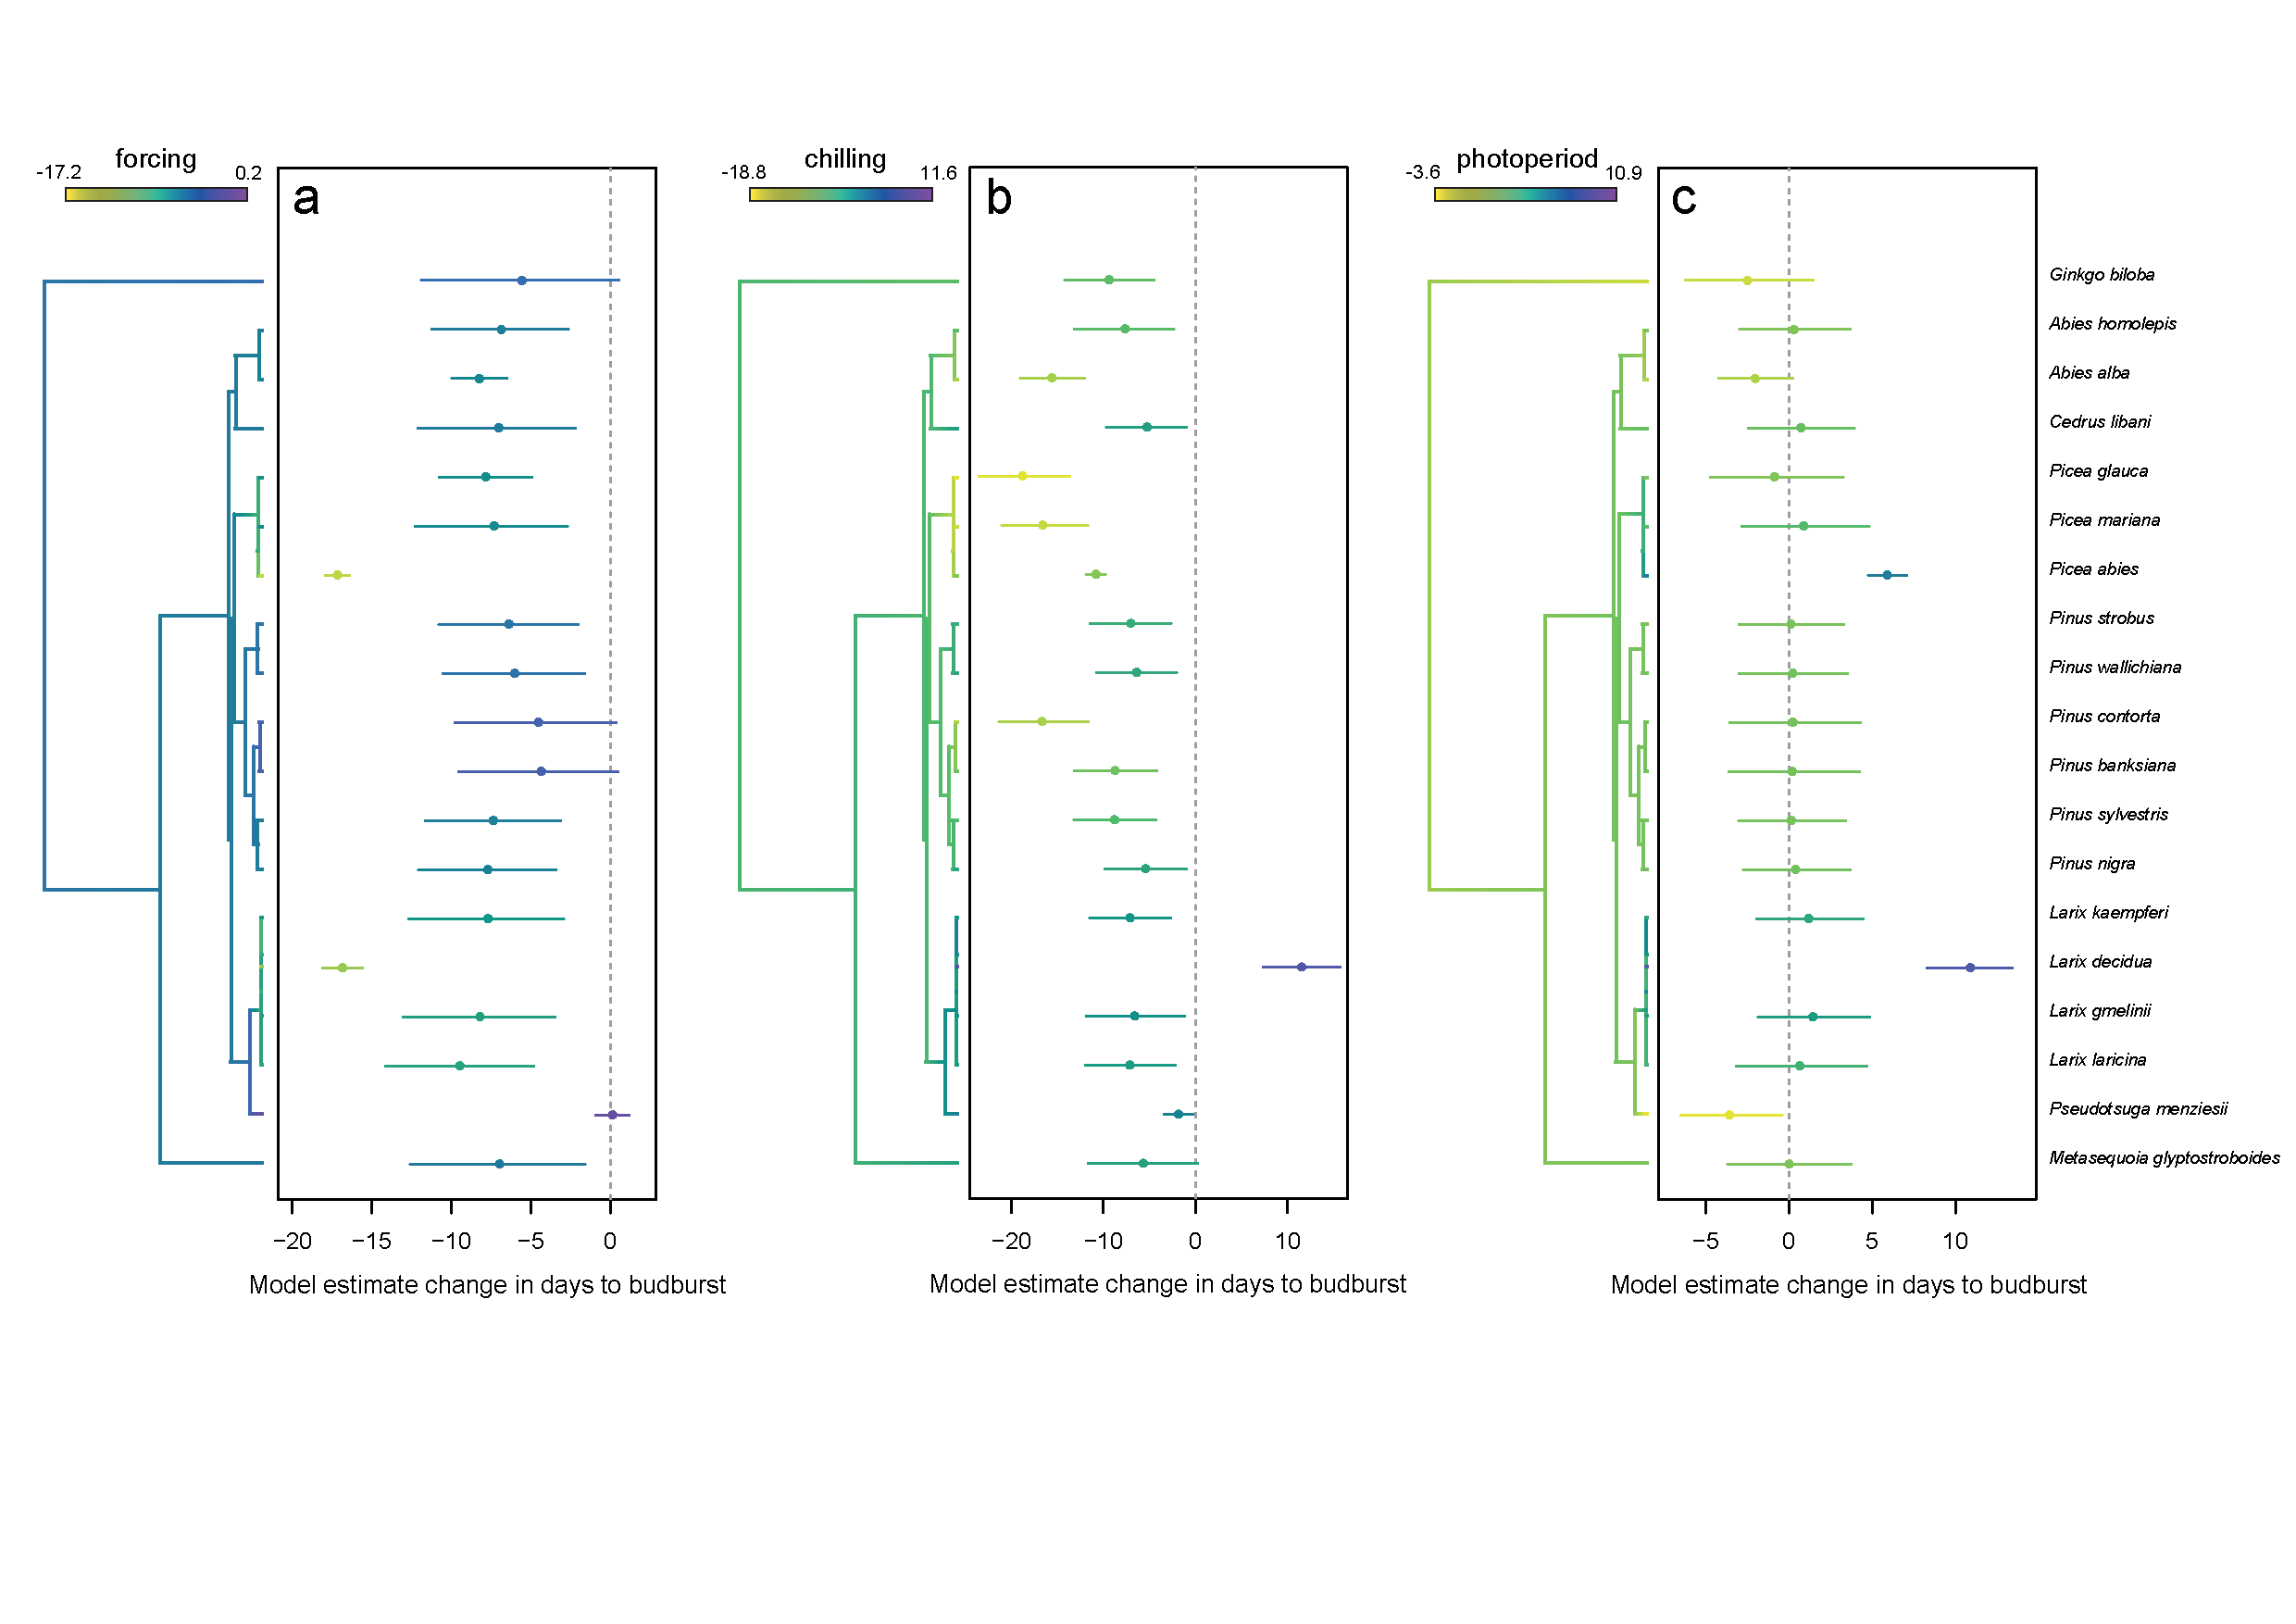
\includegraphics[width=16cm]{../../analyses/phylogeny/figures/Fig1b_phylo_muplots_gymno.pdf}
  \caption{Phenological sensitivity to thee environmental cues, forcing (a), chilling (b) and photoperiod (c) measured in change in days to budburst per standardized unit (z-transformation) of the cues across 19 gymnosperm species. The same phylogenetic tree is shown in each panel, colored acording to an estimation of ancestral character states, being the states at the tips the model slopes of our hierarchical phylogenetic model. Note that the color scale varies in each panel. Total tree depth is 81. My.}
  \label{fig:muplot_allgymno}
  \end{center}
\end{figure}


\begin{figure} [H]
  \begin{center}
  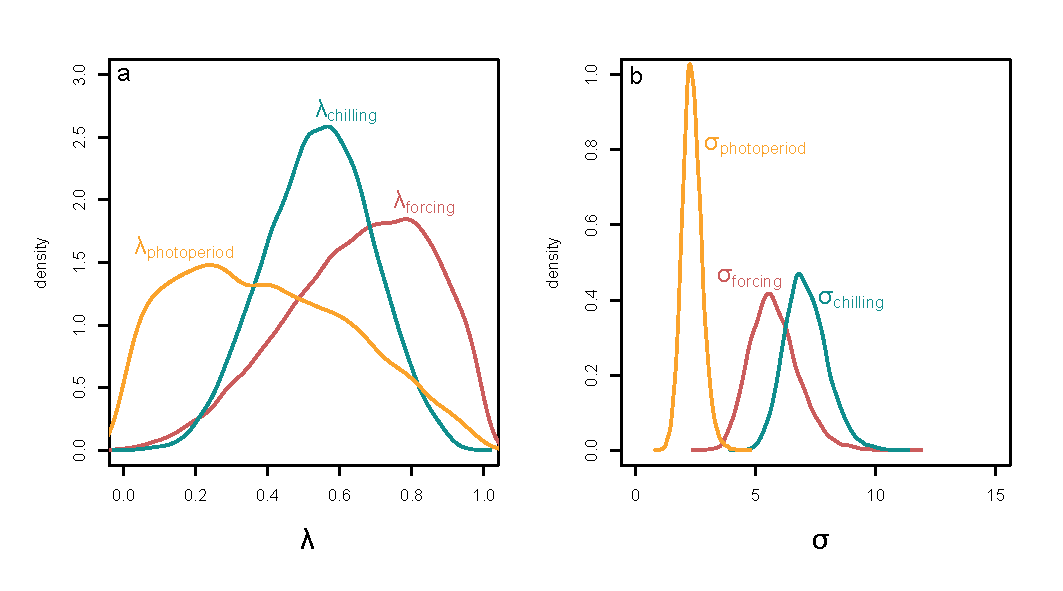
\includegraphics[width=14cm]{../../analyses/phylogeny/figures/Fig2_lambdas_sigmas.pdf}
  \caption{Density plots for the posterior distribution of phylogenetic signal measured by lambda for each cue included as a predictor in the model for angiosperms: forcing (red), chilling (blue),  photoperiod (orange) and for the model intercept (grey). Panels correspond to angiosperms (a-d) and gymnosperms (e-h). Note that lambda estimations corresponding to  panels c-d and g-h as they are constrained to be either equal zero or equal 1.}
  \label{fig:phylosig_all}
  \end{center}
\end{figure}

\begin{figure} [H]
  \begin{center}
  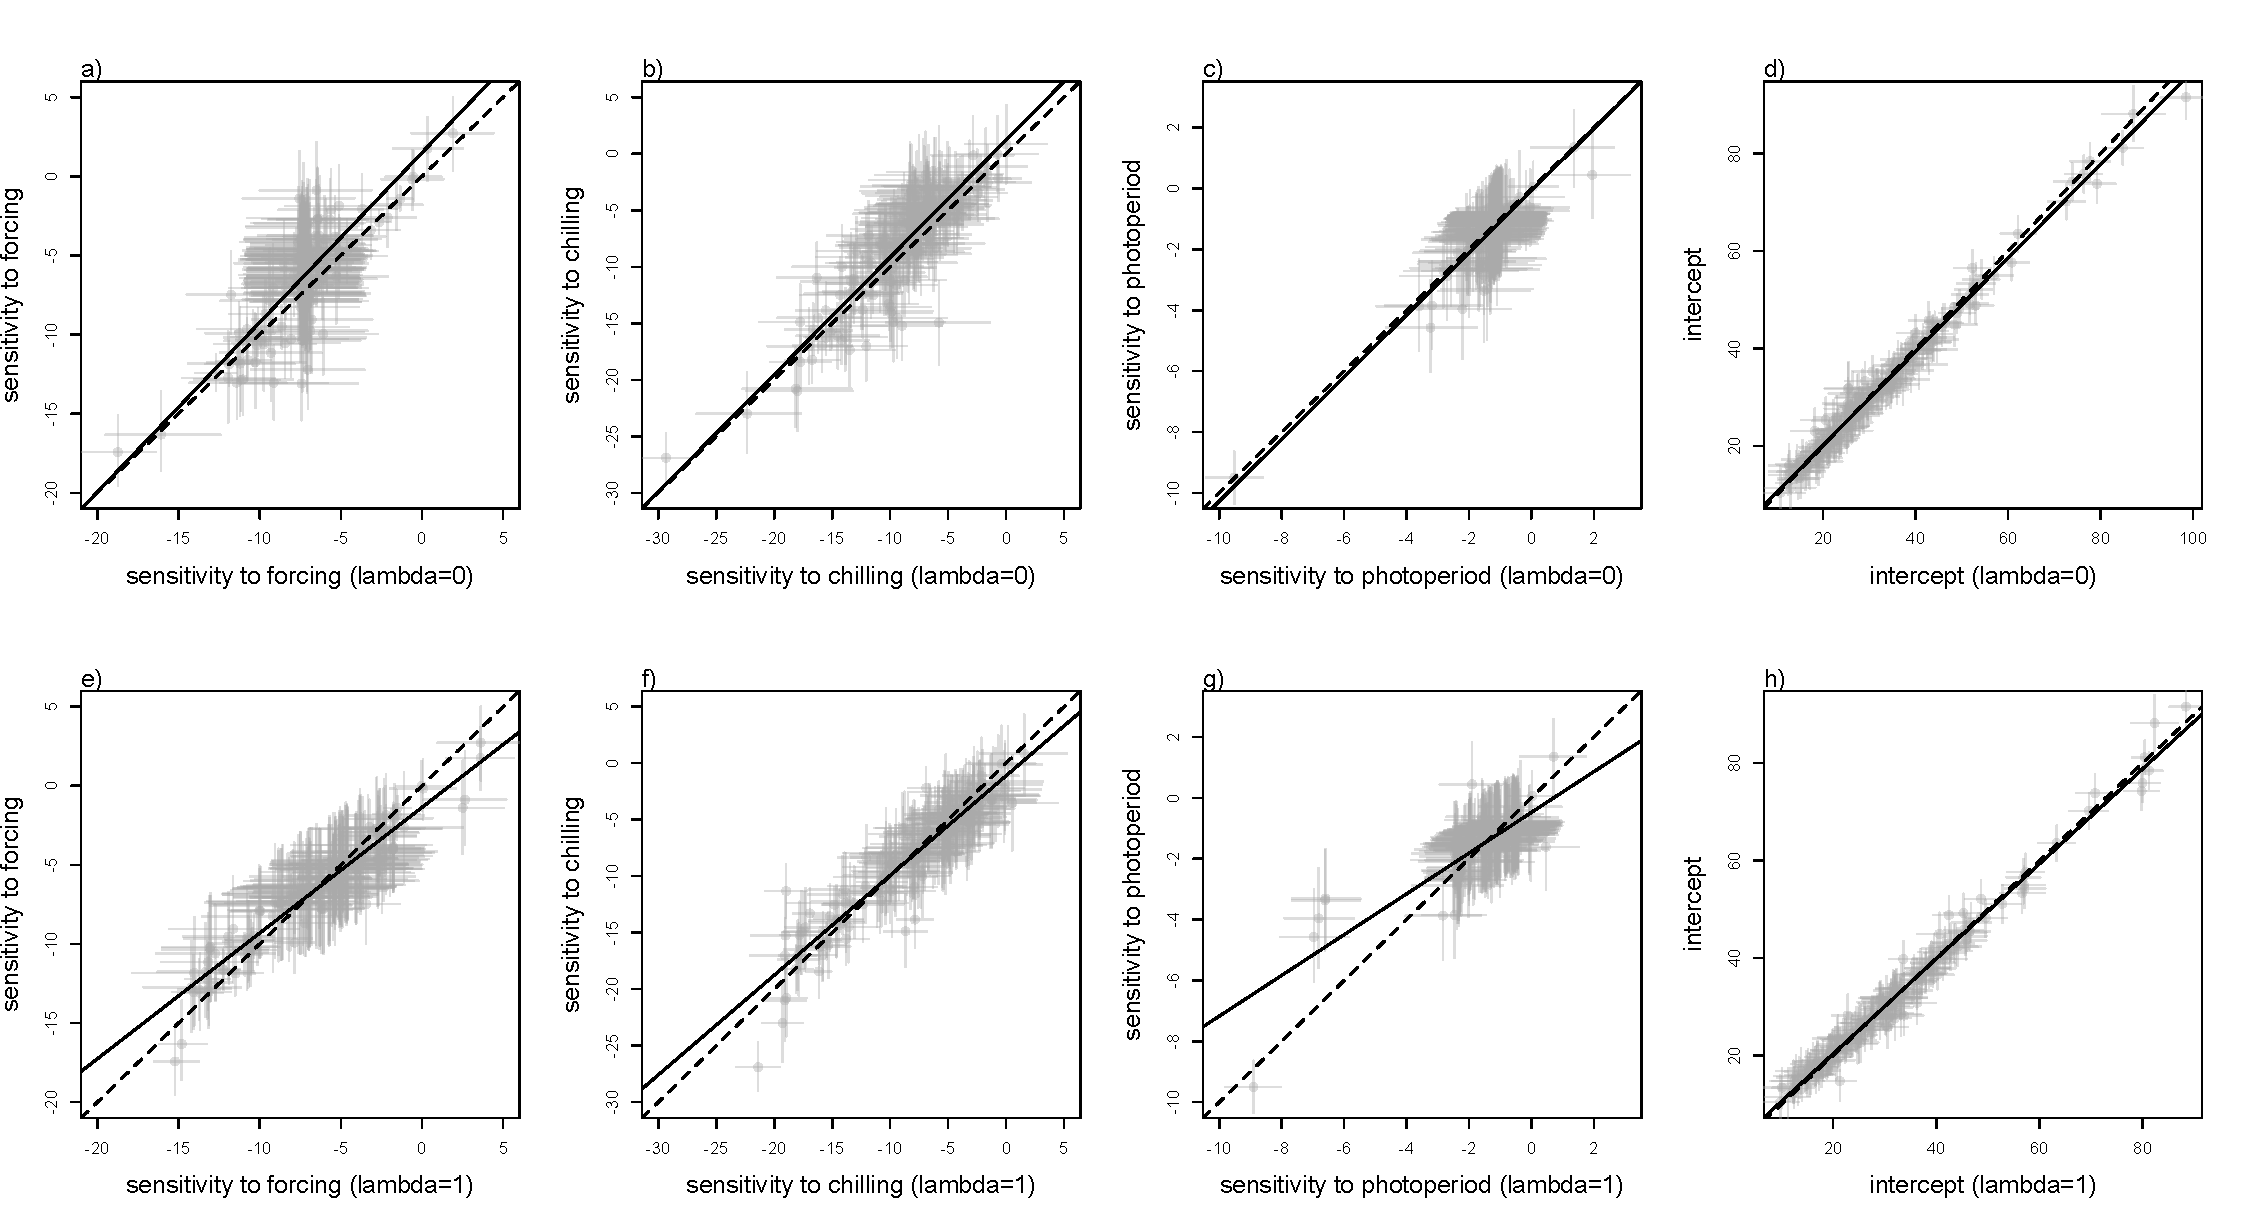
\includegraphics[width=14cm]{../../analyses/phylogeny/figures/Est_correls_vs_lamb01_angio.pdf}
  \caption{Correlations between model parameters as estimated by the full model and the models where lambda is constrained to be equal zero (upper row) or one (bottom row), for angiosperms. Panels correspond to sensitivity to forcing (a,e), to chilling (b,f), to photoperiod (c,g) and to model intercepts (d,h).}
  \label{fig:correls_angio}
  \end{center}
\end{figure}

\begin{figure} [H]
  \begin{center}
  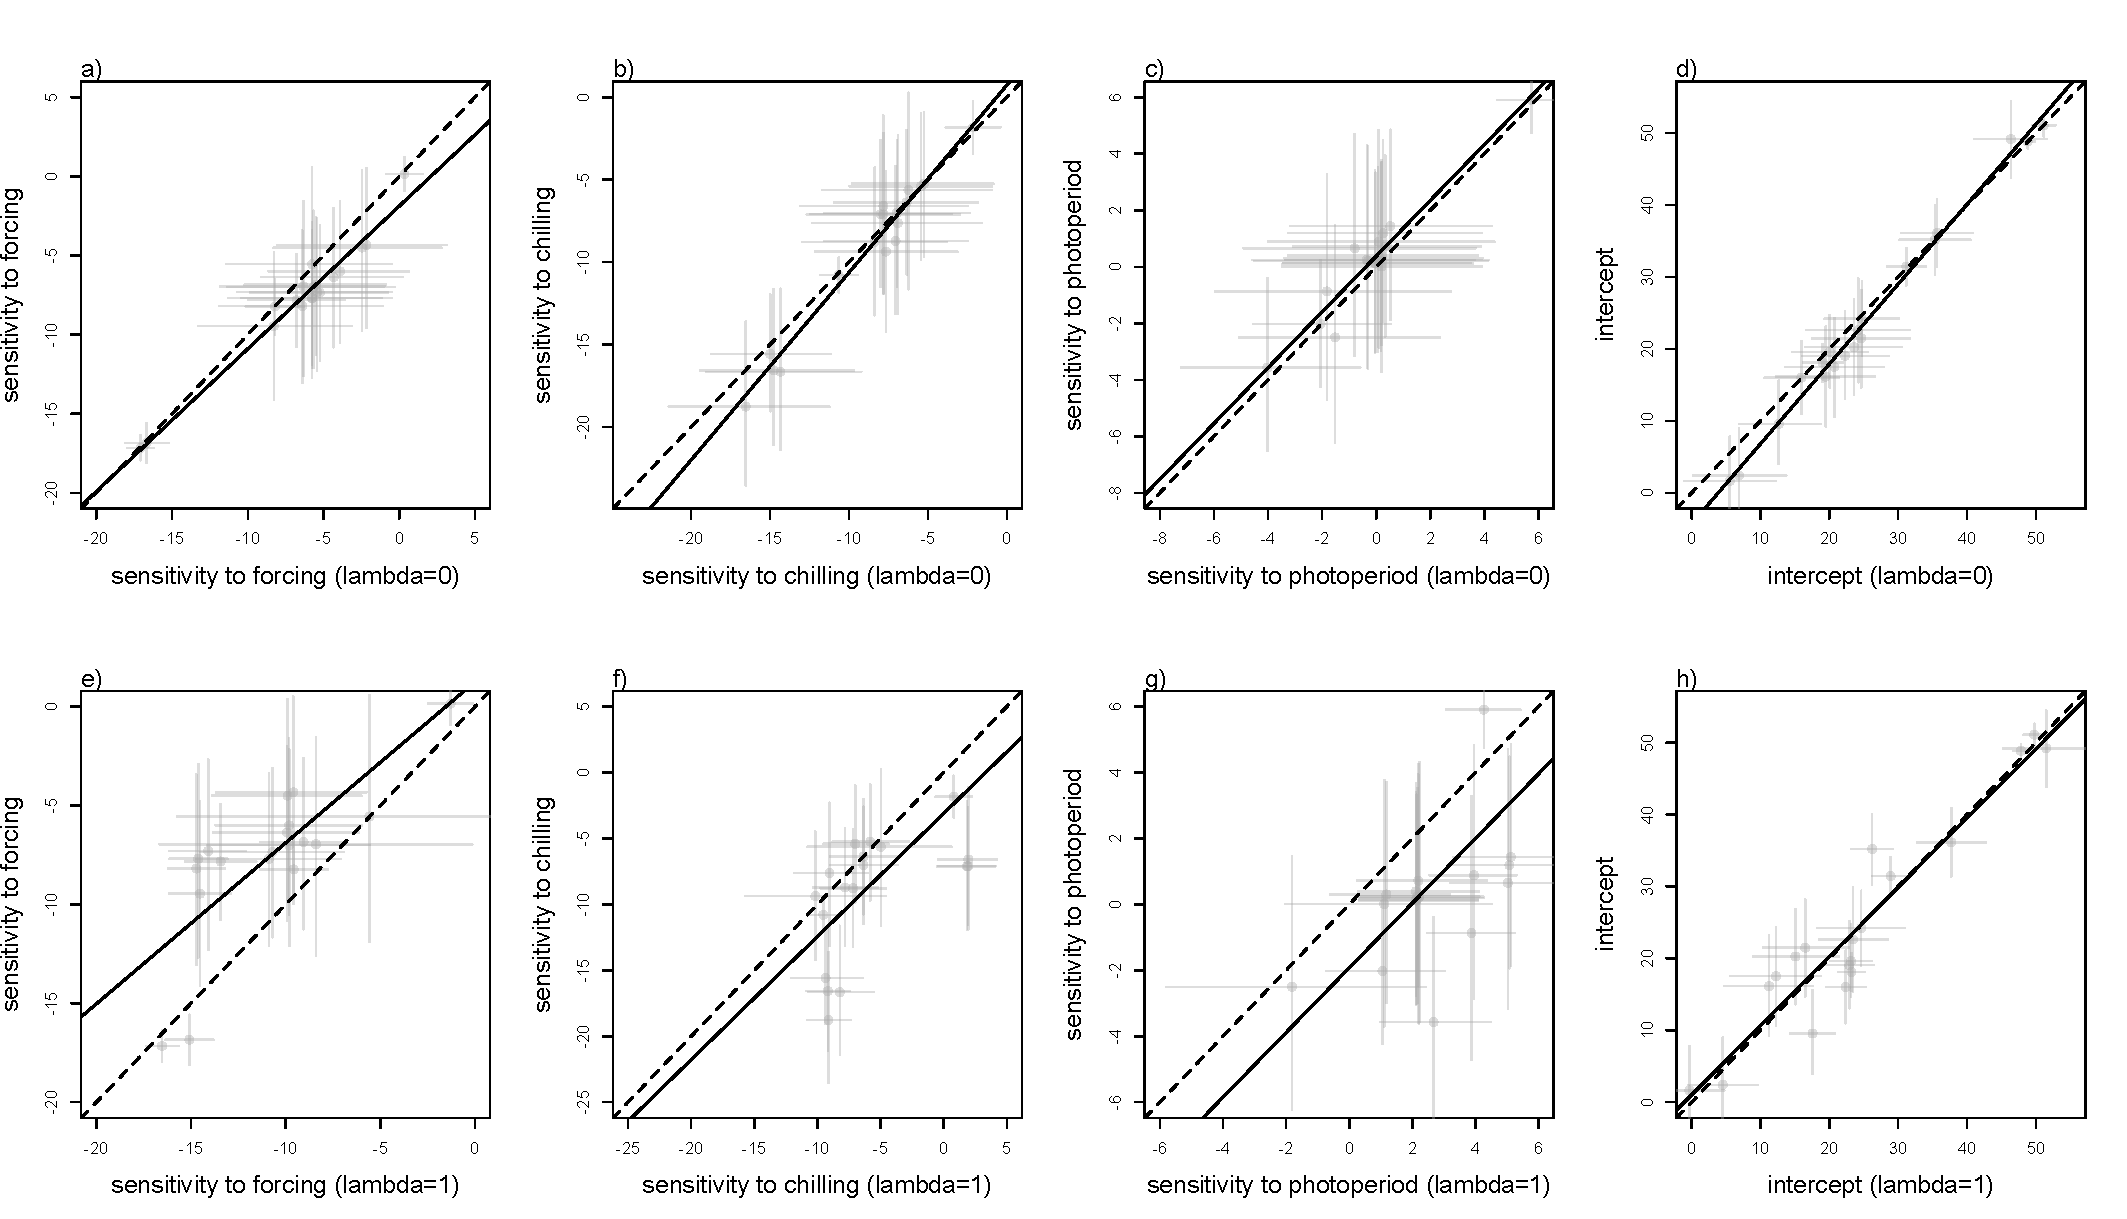
\includegraphics[width=14cm]{../../analyses/phylogeny/figures/Est_correls_vs_lamb01_gymno.pdf}
  \caption{Correlations between model parameters as estimated by the full model and the models where lambda is constrained to be equal zero (upper row) or one (bottom row), for gymnosperms. Panels correspond to sensitivity to forcing (a,e), to chilling (b,f), to photoperiod (c,g) and to model intercepts (d,h).}
  \label{fig:correls_gymno}
  \end{center}
\end{figure}



\begin{table}[H]
\begin{center}
\caption{Full model parameters estimated for 192 angiosperm species.}
\begin{tabular}{@{}lcccccc@{}}                      
\end{tabular}
\end{center}
\label{tab:modelanglamb}
\end{table}


\begin{table}[H]
 \begin{center}
\caption{Full model parameters estimated for 19 gymnosperm species.}
\begin{tabular}{@{}lcccccc@{}}
\end{tabular}
\end{center}
\label{tab:modelgymlamb}
\end{table}


\end{document}
